%To compile as handout, use
%pdflatex "\def\ishandout{1} \input{filename.tex}"
%Defaults to non-handout mode (with slide reveals)
\ifdefined\ishandout
  \documentclass[handout]{beamer}
\else
  \documentclass{beamer}
\fi
 
\usepackage{econ103slides} 

\date{Lecture 21}


\begin{document} 




%%%%%%%%%%%%%%%%%%%%%%%%%%%%%%%%%%%%%%%%

\begin{frame}[plain]
	\titlepage 
	

\end{frame} 


%%%%%%%%%%%%%%%%%%%%%%%%%%%%%%%%%%%%%%%%

\begin{frame}
\begin{center}
	\huge Hypothesis Testing -- Part II
\end{center}
\end{frame}

%%%%%%%%%%%%%%%%%%%%%%%%%%%%%%%%%%%%%%%%
%\begin{frame}
%\frametitle{Central Idea of Hypothesis Testing: Control Type I Errors}
%\pause
%	\begin{enumerate}
%		\item Choose significance level $\alpha$ \pause
%			\begin{itemize} 
%				\item Max prob.\ of Type I error (reject true $H_0$) we will accept \pause
%			\end{itemize}
%		\item Choose a test statistic $T_n$ \pause
%			\begin{itemize}
%				\item Known sampling distribution under $H_0$ \pause
%			 \end{itemize} 
%		\item Specify a decision rule involving $T_n$ and critical value $c_\alpha$ \pause
%			\begin{itemize}
%				\item Chosen to keep Type I error probability $\leq \alpha$ \pause
%				\item Typically: Reject $H_0$ if $T_n \geq c_\alpha$ \pause
%				\item (Could be $\leq$ depending on the problem) 
%			\end{itemize}
%	\end{enumerate}
%\end{frame}


%%%%%%%%%%%%%%%%%%%%%%%%%%%%%%%%%%%%%%%%
\begin{frame}
\begin{block}{Last Time}
Simple Example of Hypothesis Testing: the Pepsi Challenge
\end{block}

\begin{block}{Today}
Hypothesis Testing More Generally
\end{block}

\end{frame}
%%%%%%%%%%%%%%%%%%%%%%%%%%%%%%%%%%%%%%%%
\begin{frame}

\begin{alertblock}{Step 1}
Specify the Null and Alternative Hypotheses.
\end{alertblock}

\end{frame}

%%%%%%%%%%%%%%%%%%%%%%%%%%%%%%%%%%%%%%%%
\begin{frame}
\frametitle{Hypotheses Are Assertions about Population Parameters}
\begin{block}{For Example:}
	\begin{itemize}
		\item Population mean is zero ($\mu = 0$)
		\item Population proportion is 50\% ($p=0.5$) 
		% \item Population Variance greater than 5 ($\sigma^2 > 5$) 
		% \item Proportion in first popn.\ greater than in second $(p - q \geq 0)$ 
		\item The means of two populations are equal $(\mu_x = \mu_y)$ 
	\end{itemize}
	
	\end{block}
\end{frame}
%%%%%%%%%%%%%%%%%%%%%%%%%%%%%%%%%%%%%%%%
\begin{frame}
\frametitle{For This Course: Simple Null Hypotheses}
	Our null hypotheses will always take the form $H_0\colon \theta = \theta_0$ where $\theta$ is a population parameter and $\theta_0$ is \alert{some specified value}, e.g.\ 3.\\ 
	 
	\vspace{2em}
	\alert{What will differ depending on the situation is the alternative hypothesis...}
\end{frame}


%%%%%%%%%%%%%%%%%%%%%%%%%%%%%%%%%%%%%%%%
\begin{frame}
\frametitle{One-sided vs.\ Two-sided Alternative}
\alert{In each case the null hypothesis is $H_0\colon \theta = \theta_0$}
	\begin{block}{Two-sided Alternative}
		\begin{itemize}
			\item $H_1\colon \theta \neq \theta_0$
		\end{itemize}
\end{block}
	\begin{block}{One-sided Alternative}
		Two possibilities, depending on the problem at hand:
		\begin{itemize}
			\item $H_1\colon \theta > \theta_0$
			\item $H_1\colon \theta < \theta_0$
		\end{itemize}
\end{block}
\end{frame}



%%%%%%%%%%%%%%%%%%%%%%%%%%%%%%%%%%%%%%%%
\begin{frame}
\frametitle{Example: Suing McDonald's}

A class action lawsuit claims that McDonald's has been  understating the caloric content of the ``Big Mac,'' misleading consumers into thinking the sandwich is healthier than it really is. McDonald's claims the sandwich contains $550$ kcal on average. \\

\vspace{1em}
Presumably there's some variation, both sandwich to sandwich and in the device used to measure calories, so we should interpret this as a claim about the \alert{population mean} caloric content of the sandwich ($\mu$).
\end{frame}


%%%%%%%%%%%%%%%%%%%%%%%%%%%%%%%%%%%%%%%%

\begin{frame}
\frametitle{Example: Suing McDonald's \hfill 
\includegraphics[scale = 0.05]{./images/clicker}}

A class action lawsuit claims that McDonald's has been  understating the caloric content of the ``Big Mac,'' misleading consumers into thinking the sandwich is healthier than it really is. McDonald's claims the sandwich contains $550$ kcal on average. \\

\vspace{1em}
\alert{Suppose you're the judge in this case. What is your null hypothesis?}

	\begin{enumerate}[(a)]
		\item $H_0\colon \mu \neq 550$ kcal
		\item $H_0\colon \mu < 550$ kcal
		\item $H_0\colon \mu > 550$ kcal
		\item $H_0\colon \mu = 550$ kcal
\end{enumerate}
\end{frame}
%%%%%%%%%%%%%%%%%%%%%%%%%%%%%%%%%%%%%%%%

\begin{frame}
\frametitle{Example: Suing McDonald's \hfill 
\includegraphics[scale = 0.05]{./images/clicker}}

A class action lawsuit claims that McDonald's has been  understating the caloric content of the ``Big Mac,'' misleading consumers into thinking the sandwich is healthier than it really is. McDonald's claims the sandwich contains $550$ kcal on average. \\

\vspace{1em}
\alert{Suppose you're the judge in this case. What is your alternative hypothesis?}

	\begin{enumerate}[(a)]
		\item $H_1\colon \mu \neq 550$ kcal
		\item $H_1\colon \mu < 550$ kcal
		\item $H_1\colon \mu > 550$ kcal
		\item $H_1\colon \mu = 550$ kcal
\end{enumerate}
\end{frame}
%%%%%%%%%%%%%%%%%%%%%%%%%%%%%%%%%%%%%%%%
\begin{frame}
\frametitle{Example: Quality Control at McDonald's}

You are a senior manager at McDonald's and are concerned that franchises may be deviating from company policy on the calorie count of a Big Mac sandwich, which is supposed to be 550 kcal on average. Because intervening is costly, you will only take action is there is strong evidence of deviation company policy. 

\end{frame}
%%%%%%%%%%%%%%%%%%%%%%%%%%%%%%%%%%%%%%%%
\begin{frame}
\frametitle{Example: Quality Control at McDonald's \hfill 
\includegraphics[scale = 0.05]{./images/clicker}}

You are a senior manager at McDonald's and are concerned that franchises may be deviating from company policy on the calorie count of a Big Mac sandwich, which is supposed to be 550 kcal on average. Because intervening is costly, you will only take action is there is strong evidence of deviation company policy. \\

\vspace{1em}

\alert{What is your null hypothesis?}
	\begin{enumerate}[(a)]
		\item $H_0\colon \mu \neq 550$ kcal
		\item $H_0\colon \mu < 550$ kcal
		\item $H_0\colon \mu > 550$ kcal
		\item $H_0\colon \mu = 550$ kcal
\end{enumerate}
\end{frame}


%%%%%%%%%%%%%%%%%%%%%%%%%%%%%%%%%%%%%%%%
\begin{frame}
\frametitle{Example: Quality Control at McDonald's \hfill 
\includegraphics[scale = 0.05]{./images/clicker}}

You are a senior manager at McDonald's and are concerned that franchises may be deviating from company policy on the calorie count of a Big Mac sandwich, which is supposed to be 550 kcal on average. Because intervening is costly, you will only take action is there is strong evidence of deviation company policy. \\

\vspace{1em}

\alert{What is your alternative hypothesis?}
	\begin{enumerate}[(a)]
		\item $H_1\colon \mu \neq 550$ kcal
		\item $H_1\colon \mu < 550$ kcal
		\item $H_1\colon \mu > 550$ kcal
		\item $H_1\colon \mu = 550$ kcal
\end{enumerate}
\end{frame}
% %%%%%%%%%%%%%%%%%%%%%%%%%%%%%%%%%%%%%%%%
% \begin{frame}
% \frametitle{Example: Bias in Jury Selection \hfill 
\includegraphics[scale = 0.05]{./images/clicker}}
% You are investigating a judge who is suspected of showing bias against women in jury selection. Of the 700 jury members he has selected only $15\%$ were women. In contrast, $29\%$ of eligible jurors were women. Let $p$ be the probability that a juror drawn by this judge is a woman.\\

% \vspace{1em}

% \alert{What should our null hypothesis be in this case?}

% \begin{enumerate}[(a)]
% 	\item $H_0\colon p = 0.5$
% 	\item $H_0\colon p = 0.29$
% 	\item $H_0\colon p = 0.15$
% 	\item $H_0\colon p \neq 0.29$
% \end{enumerate}

% \end{frame}

% %%%%%%%%%%%%%%%%%%%%%%%%%%%%%%%%%%%%%%%%
% \begin{frame}
% \frametitle{Example: Bias in Jury Selection \hfill 
\includegraphics[scale = 0.05]{./images/clicker}}
% You are investigating a judge who is suspected of showing bias against women in jury selection. Of the 700 jury members he has selected only $15\%$ were women. In contrast, $29\%$ of eligible jurors were women. Let $p$ be the probability that a juror drawn by this judge is a woman.\\

% \vspace{1em}

% \alert{What should our alternative hypothesis be in this case?}

% \begin{enumerate}[(a)]
% 	\item $H_1\colon p \neq 0.29$
% 	\item $H_1\colon p \neq 0.15$
% 	\item $H_1\colon p < 0.29$
% 	\item $H_1\colon p > 0.29$
% \end{enumerate}

% \end{frame}

% %%%%%%%%%%%%%%%%%%%%%%%%%%%%%%%%%%%%%%%%

\begin{frame}
\begin{center}
\huge Which alternative to use depends on the problem at hand.
\end{center}
\end{frame}

%%%%%%%%%%%%%%%%%%%%%%%%%%%%%%%%%%%%%%%%

\begin{frame}
\begin{alertblock}{Step 2}
Identify a \emph{Test Statistic}: a function of the data and the unknown parameter that has a \emph{known sampling distribution if $H_0$ is true} (i.e.\ ``Under the Null'').
\end{alertblock}
\end{frame}

%%%%%%%%%%%%%%%%%%%%%%%%%%%%%%%%%%%%%%%%

\begin{frame}
\frametitle{The Two McDonald's Examples}
Suppose we take a random sample of $n$ Big Macs and measure their caloric content: $X_1, \hdots, X_n \sim \mbox{iid} (\mu, \sigma^2)$

\begin{block}{Lawsuit: One-sided Alternative}
$H_0\colon \mu = 550$\\
$H_1\colon \mu > 550$
\end{block}
\begin{block}{Quality Control: Two-sided Alternative}
$H_0\colon \mu = 550$\\
$H_1\colon \mu \neq 550$
\end{block}
\alert{What test statistic has a known distribution under the null?}
\end{frame}

%%%%%%%%%%%%%%%%%%%%%%%%%%%%%%%%%%%%%%%%
\begin{frame}
\frametitle{What Test Statistic to Use?}
Suppose we take a random sample of $n$ Big Macs and measure their caloric content: $X_1, \hdots, X_n \sim \mbox{iid} (\mu, \sigma^2)$

\begin{block}{Possibility I: Assume the Population is Normal}
 $$H_0\colon \mu = 550 \Rightarrow \displaystyle \frac{\bar{X}_n - 550}{S/\sqrt{n}}\sim t(n-1)$$
\end{block}

\begin{block}{Possibility II: Assume $n$ is large and use CLT}
 $$H_0\colon \mu = 550 \Rightarrow \displaystyle \frac{\bar{X}_n - 550}{S/\sqrt{n}}\approx N(0,1)$$
\end{block}

\alert{Same basic idea in each case. I'll show you the first one.}
\end{frame}


%%%%%%%%%%%%%%%%%%%%%%%%%%%%%%%%%%%%%%%%

\begin{frame}
\begin{alertblock}{Step 3}
Specify a \emph{Decision Rule} and a \emph{Critical Value} so that if $H_0$ is true (i.e.\ ``Under the Null'') the probability of rejecting equals $\alpha$, a \emph{user specified Type I Error Rate}.
\end{alertblock}
\end{frame}

%%%%%%%%%%%%%%%%%%%%%%%%%%%%%%%%%%%%%%%%


\begin{frame}
\frametitle{What Form Should the Decision Rule Take?}
\begin{columns}
\begin{column}[l]{6cm}
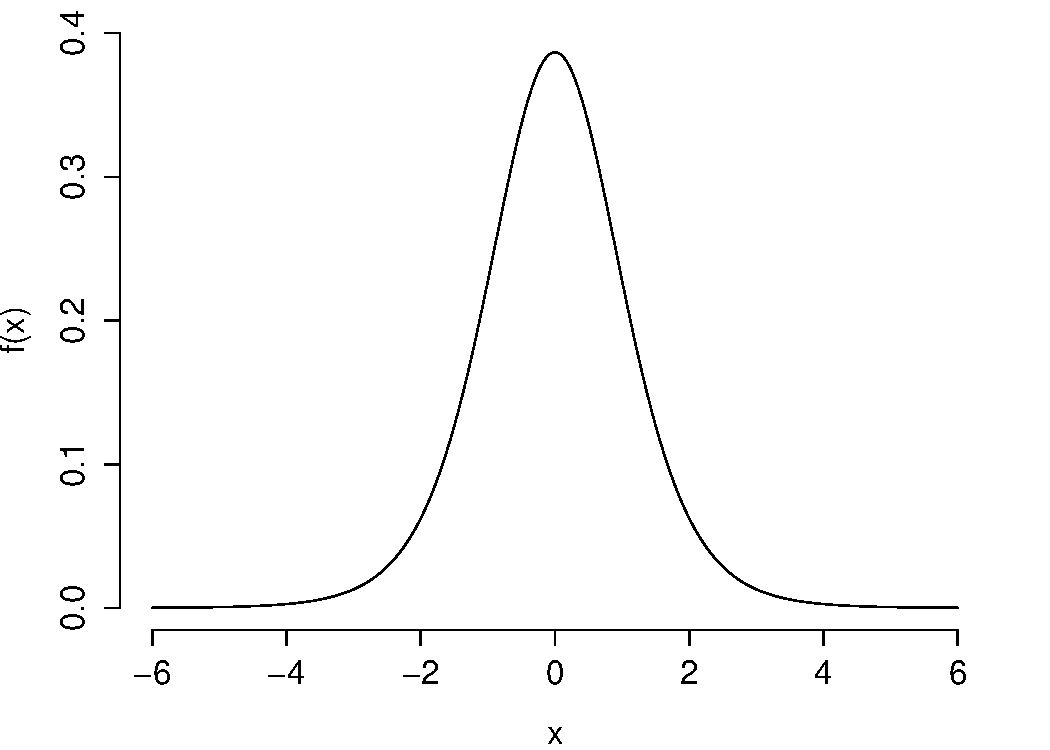
\includegraphics[scale = 0.5]{./images/t_pdf}
\end{column}

\begin{column}[r]{6cm}
$H_0\colon \mu=550 \Rightarrow \displaystyle \frac{\bar{X}_n - 550}{S/\sqrt{n}} \sim t(n-1)$\\ \pause
\vspace{1em}
One-sided Alternative $H_1\colon \mu > 550$\\ \pause
\vspace{1em}
Two-sided Alternative $H_1\colon \mu \neq 550$ 
\end{column}

\end{columns}
 
\end{frame}
%%%%%%%%%%%%%%%%%%%%%%%%%%%%%%%%%%%%%%%%


\begin{frame}
\frametitle{What Form Should the Decision Rule Take?}
Suppose we take a random sample of $n$ Big Macs and measure their caloric content. Assume that the population is normal: $X_1, \hdots, X_n \sim \mbox{iid } N(\mu, \sigma^2)$ 
\begin{block}{Common Null Hypothesis $H_0\colon \mu = 550$}
Under $H_0$, $T_n = \sqrt{n}(\bar{X}_n - 550)/S \sim t(n-1)$ 
\end{block}
\begin{block}{One-sided Alternative $H_1\colon \mu > 550$}
Reject $H_0$ if $T_n$ is ``too big'' 
\end{block}
\begin{block}{Two-sided Alternative $H_1\colon \mu \neq 550$} 
Reject $H_0$ if $T_n$ is ``too big'' or ``too small''
\end{block}
\end{frame}

%%%%%%%%%%%%%%%%%%%%%%%%%%%%%%%%%%%%%%%%
\begin{frame}
\frametitle{One-sided Alternative $H_1\colon \mu > 550$}
The critical value is chosen to reflect both the alternative hypothesis and the significance level. 
\begin{figure}
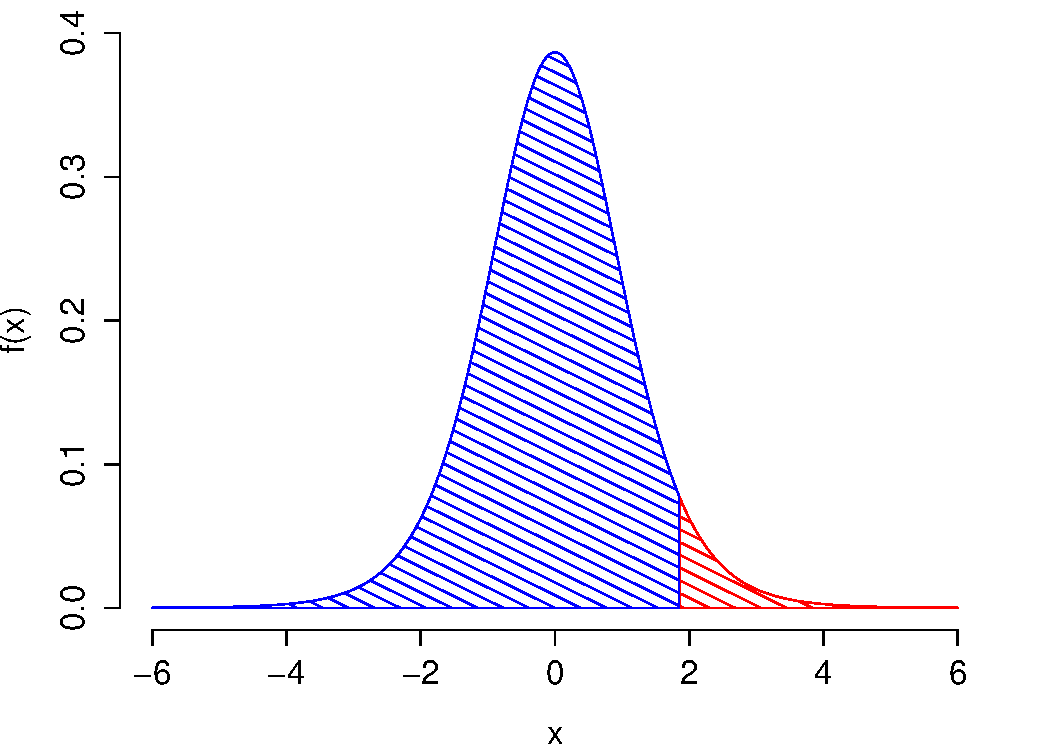
\includegraphics[scale = 0.45]{./images/one_side}
\end{figure}
One-sided Critical Value: \texttt{qt($1-\alpha$, df  = $n-1$)}
\end{frame}


%%%%%%%%%%%%%%%%%%%%%%%%%%%%%%%%%%%%%%%%

\begin{frame}
\frametitle{Two-sided Alternative $H_1\colon \mu \neq 550$}
The critical value is chosen to reflect both the alternative hypothesis and the significance level. 
\begin{figure}
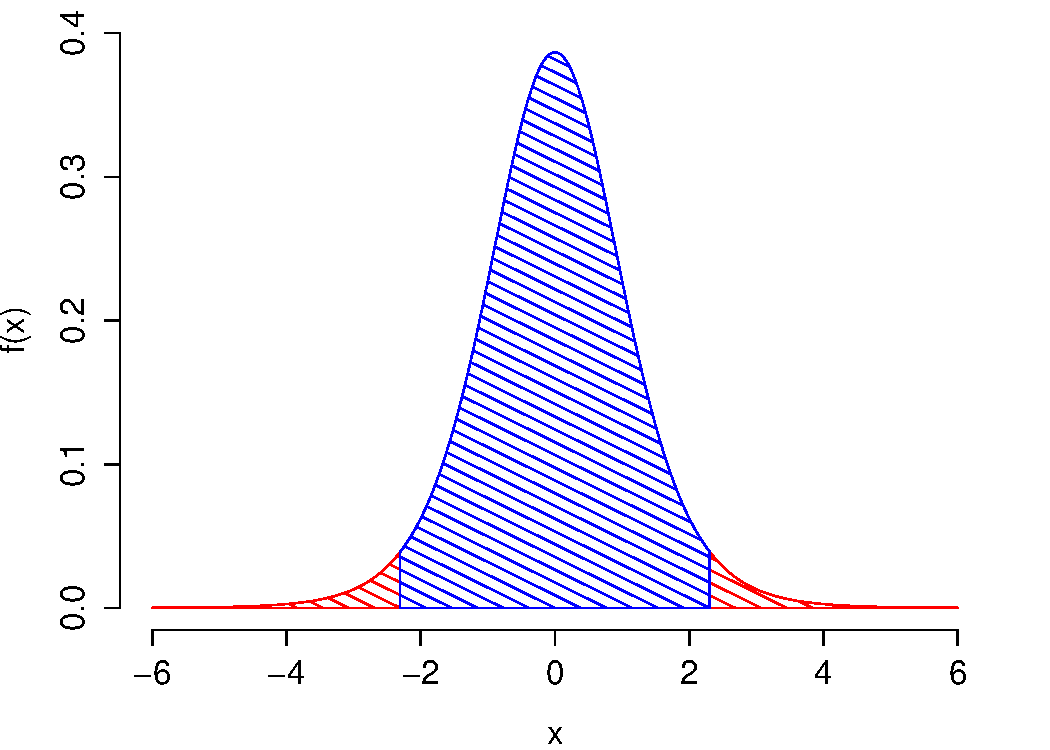
\includegraphics[scale = 0.45]{./images/two_side}
\end{figure}
Two-sided Critical Value: \texttt{qt($1-\alpha/2$, df  = $n-1$)}
\end{frame}

%%%%%%%%%%%%%%%%%%%%%%%%%%%%%%%%%%%%%%%%
\begin{frame}
Suppose, for example, $\alpha = 0.05$, $n = 9$
	\begin{eqnarray*}
		&&\texttt{qt(0.95, df  = 8)}\approx 1.86\\
		 &&\texttt{qt(0.975, df  = 8)}\approx 2.3
	\end{eqnarray*}
\begin{figure}
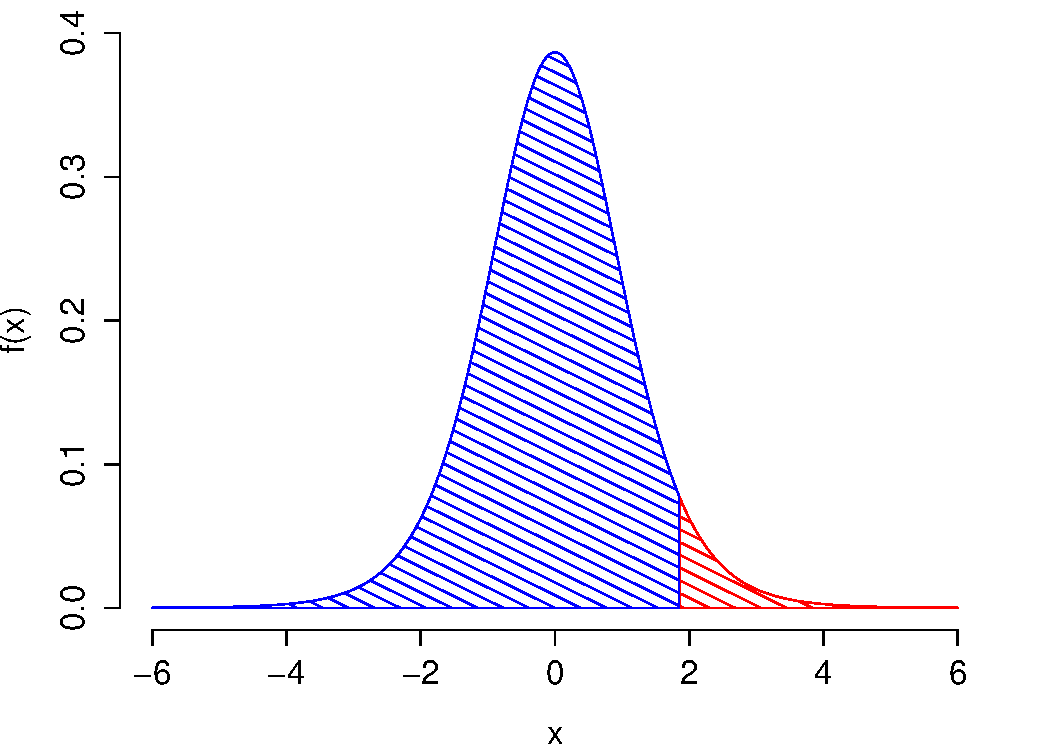
\includegraphics[scale = 0.3]{./images/one_side}
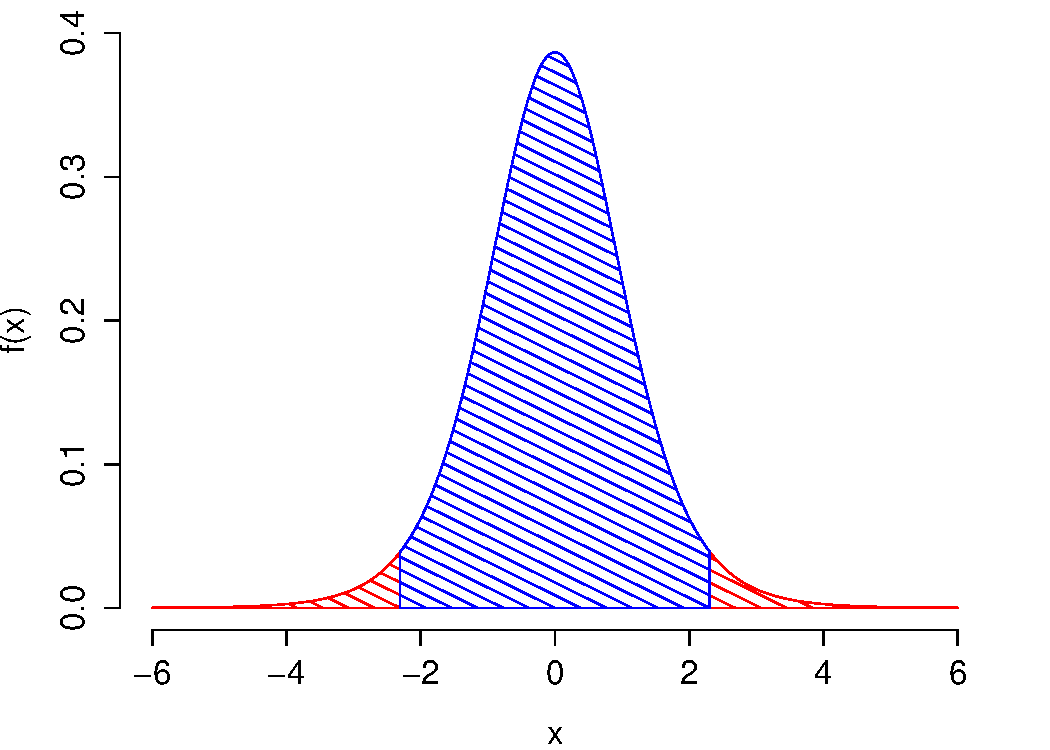
\includegraphics[scale = 0.3]{./images/two_side}
\end{figure}
One-sided Alternative: Reject $H_0$ if $\sqrt{n}(\bar{X}_n - 550)/S \geq 1.86$\\
\vspace{0.5em}
Two-sided Alternative: Reject $H_0$ if $\left|\sqrt{n}(\bar{X}_n - 550)/S\right| \geq 2.3$\\

\end{frame}

%%%%%%%%%%%%%%%%%%%%%%%%%%%%%%%%%%%%%%%%
\begin{frame}
\frametitle{Example with Simulated Data: $\alpha = 0.05$}
Suppose $n=9$, $\bar{x} = 563$, $s = 34$. What is the test statistic?


\vspace{1em}
	$$\frac{563 - 550}{34/\sqrt{9}}= \frac{13}{34/3} \approx 1.14$$



One-sided Alternative: Reject $H_0$ if $T_n\geq 1.86$\\
Two-sided Alternative: Reject $H_0$ if $\left|T_n\right| \geq 2.3$\\

\vspace{1em}
\alert{In this example, we would fail to reject $H_0$ in either case.}
\end{frame}
%%%%%%%%%%%%%%%%%%%%%%%%%%%%%%%%%%%%%%%%
\begin{frame}
\begin{center}
\huge Decision Rule and Critical Value Depend on Which Alternative We Have Specified!
\end{center}
\end{frame}

%%%%%%%%%%%%%%%%%%%%%%%%%%%%%%%%%%%%%%%%

\begin{frame}
\begin{alertblock}{Alternate Step 3}
Instead of calculating a critical value for a fixed significance level ($\alpha$), calculate the \emph{P-Value}, the minimum significance level at which we would reject the null hypothesis given the observed data.
\end{alertblock}


\end{frame}

%%%%%%%%%%%%%%%%%%%%%%%%%%%%%%%%%%%%%%%%
\begin{frame}
\frametitle{What is the p-value? (One-sided Test)}
\footnotesize
Recall: p-value is \emph{smallest significance level} at which our observed test statistic would cause us to reject $H_0$. \alert{Test statistic is $1.14$. What is the one-sided p-value? }
\begin{figure}
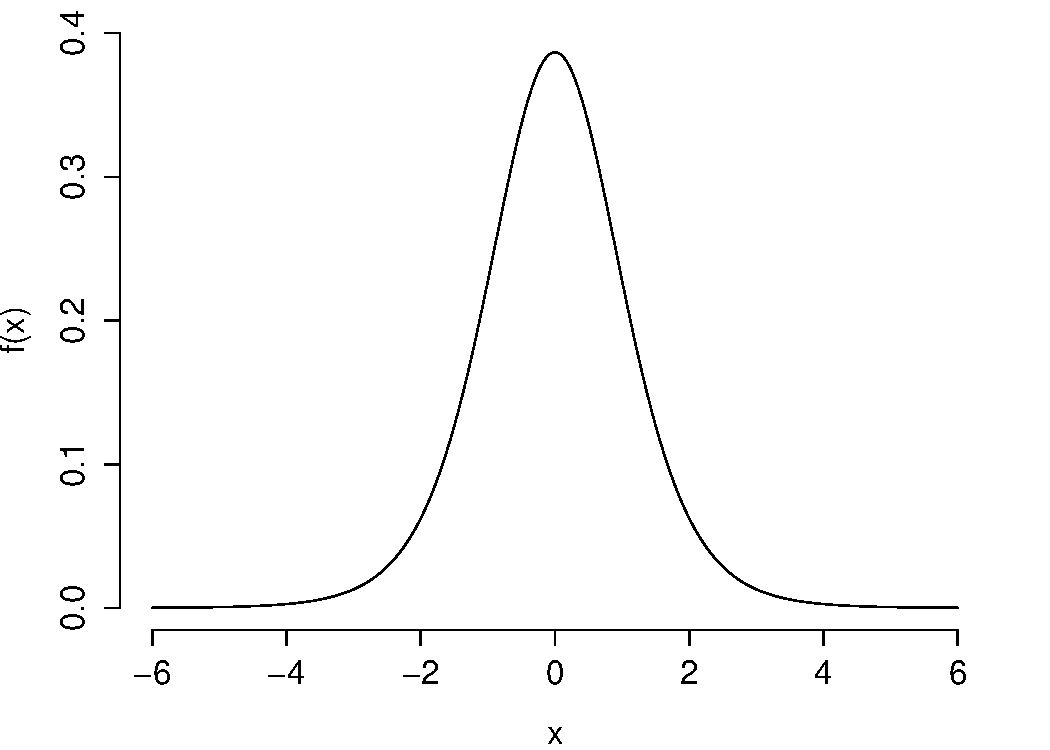
\includegraphics[scale= 0.4]{./images/p_upper1}

\end{figure}

\end{frame}

%%%%%%%%%%%%%%%%%%%%%%%%%%%%%%%%%%%%%%%%
\begin{frame}
\frametitle{What is the p-value? (One-sided Test)}
\footnotesize
Recall: p-value is \emph{smallest significance level} at which our observed test statistic would cause us to reject $H_0$. \alert{Test statistic is $1.14$. What is the one-sided p-value? }
\begin{figure}
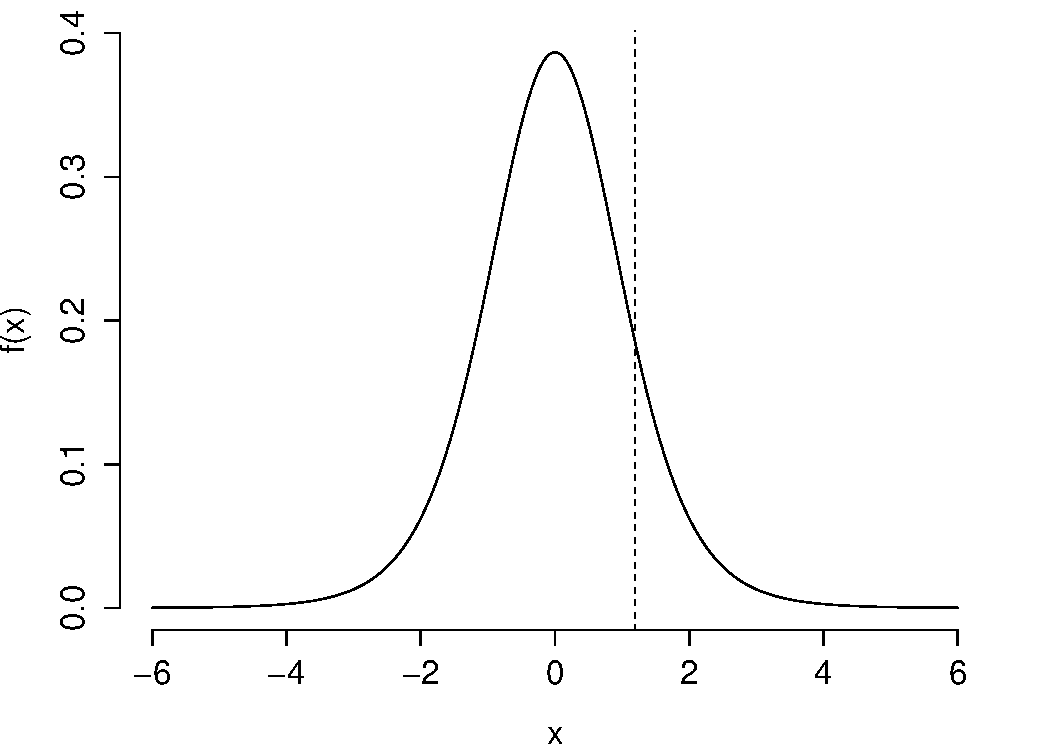
\includegraphics[scale= 0.4]{./images/p_upper2}

\end{figure}

\end{frame}

%%%%%%%%%%%%%%%%%%%%%%%%%%%%%%%%%%%%%%%%
\begin{frame}
\frametitle{What is the p-value? (One-sided Test)}
\footnotesize
Recall: p-value is \emph{smallest significance level} at which our observed test statistic would cause us to reject $H_0$. \alert{Test statistic is $1.14$. What is the one-sided p-value? }
\begin{figure}
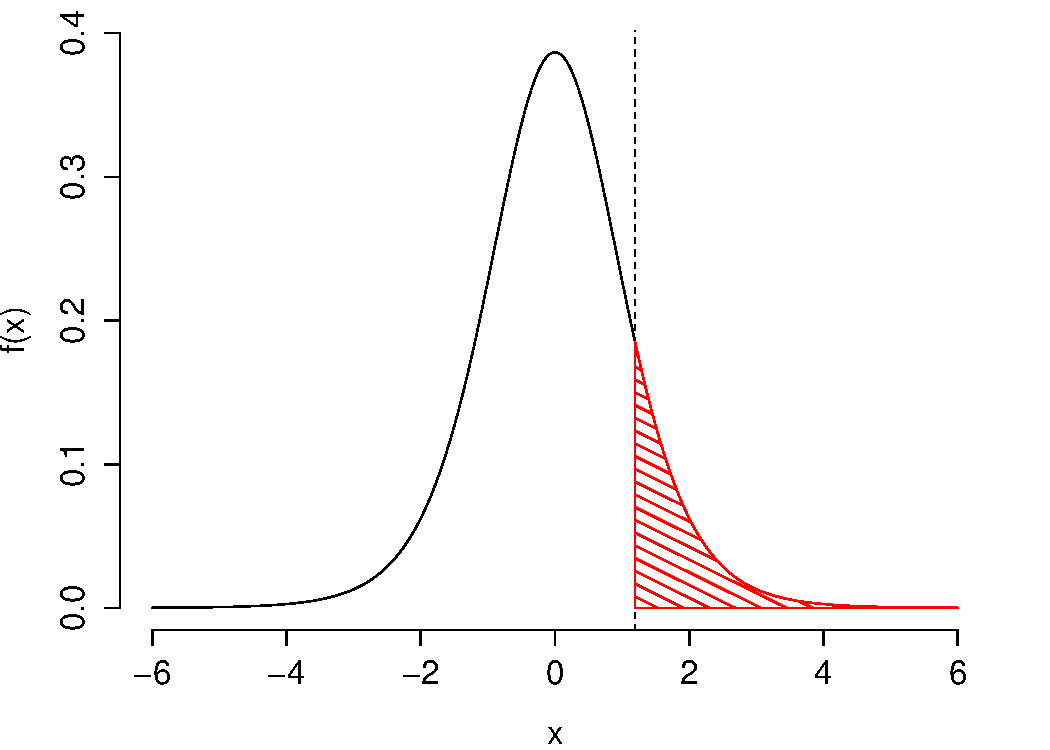
\includegraphics[scale= 0.4]{./images/p_upper3}

\end{figure}

\end{frame}

%%%%%%%%%%%%%%%%%%%%%%%%%%%%%%%%%%%%%%%%
\begin{frame}
\frametitle{What is the p-value? (One-sided Test)}
\footnotesize
Recall: p-value is \emph{smallest significance level} at which our observed test statistic would cause us to reject $H_0$. \alert{Test statistic is $1.14$. What is the one-sided p-value? }
\begin{figure}
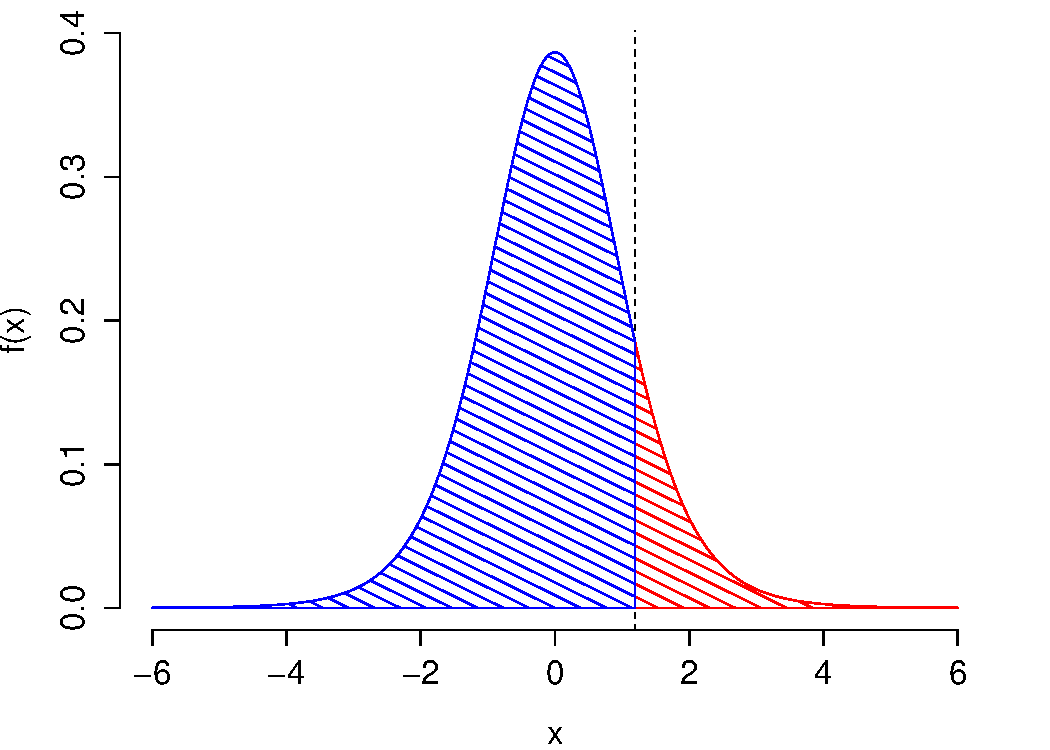
\includegraphics[scale= 0.4]{./images/p_upper4}

\end{figure}

\end{frame}

%%%%%%%%%%%%%%%%%%%%%%%%%%%%%%%%%%%%%%%%
\begin{frame}
\frametitle{What is the p-value? (One-sided Test)}
\footnotesize
Recall: p-value is \emph{smallest significance level} at which our observed test statistic would cause us to reject $H_0$. \alert{Test statistic is $1.14$. What is the one-sided p-value? }
\begin{figure}
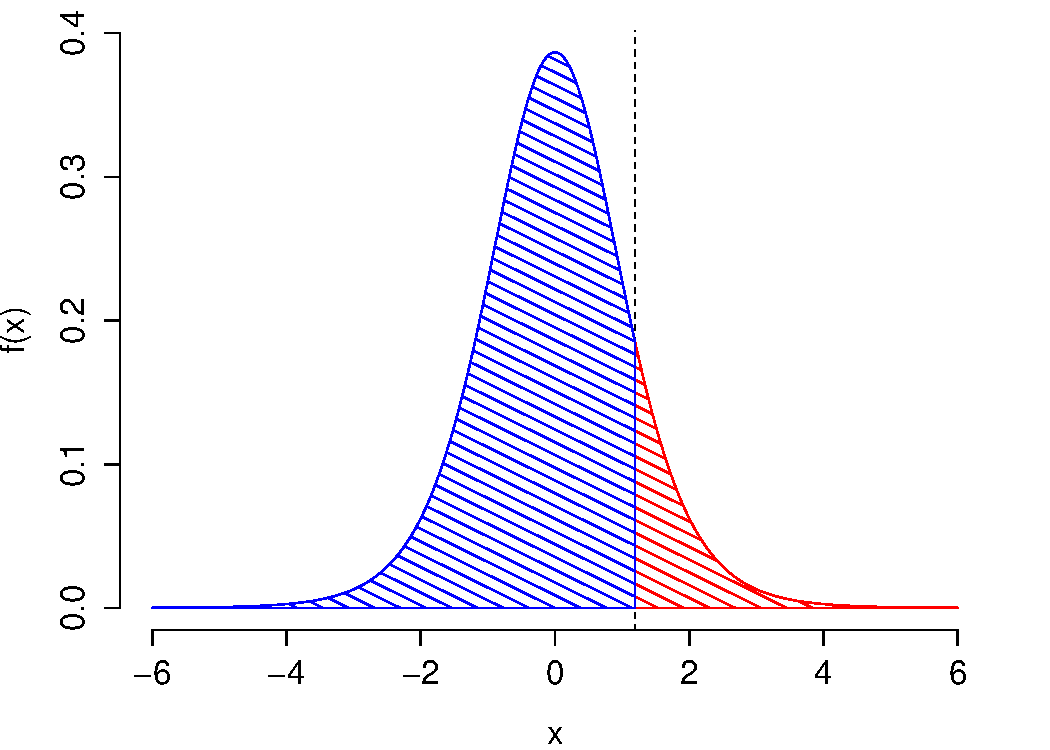
\includegraphics[scale= 0.4]{./images/p_upper4}

\end{figure}
\texttt{1 - pt(1.14, df = 8)}$\approx 0.14$
\end{frame}

%%%%%%%%%%%%%%%%%%%%%%%%%%%%%%%%%%%%%%%%
\begin{frame}
\frametitle{What is the p-value? (Two-sided Test)}
\footnotesize
Recall: p-value is \emph{smallest significance level} at which our observed test statistic would cause us to reject $H_0$. \alert{Test statistic is $1.14$. What is the two-sided p-value? }
\begin{figure}
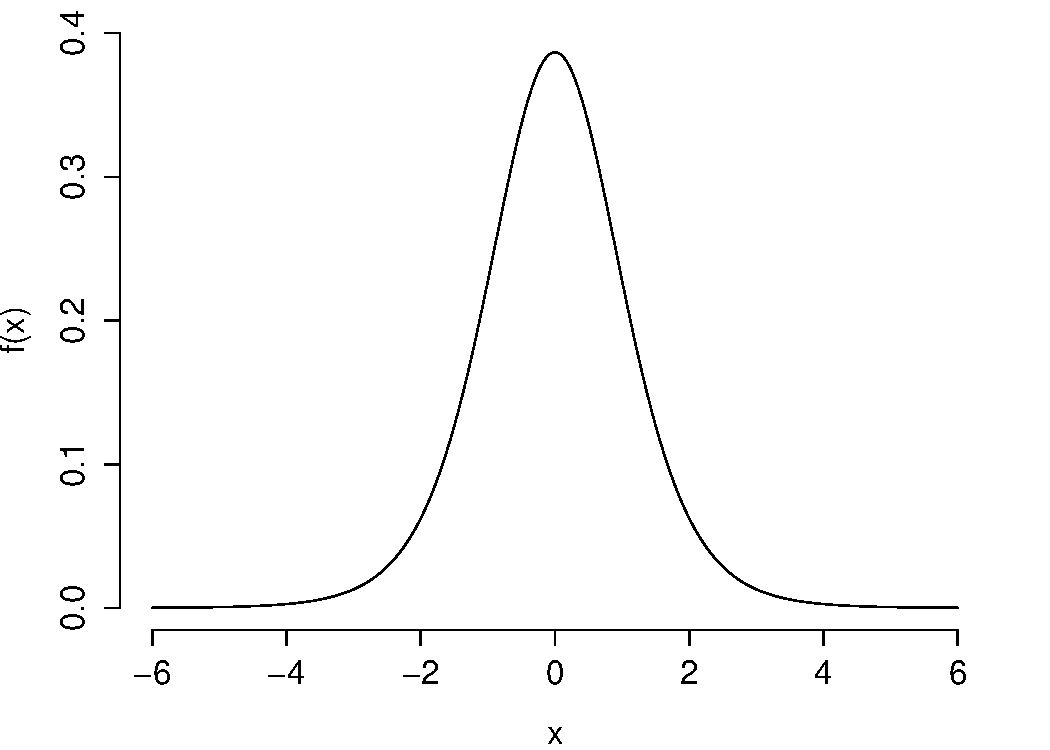
\includegraphics[scale= 0.4]{./images/p_both1}

\end{figure}

\end{frame}

%%%%%%%%%%%%%%%%%%%%%%%%%%%%%%%%%%%%%%%%
\begin{frame}
\frametitle{What is the p-value? (Two-sided Test)}
\footnotesize
Recall: p-value is \emph{smallest significance level} at which our observed test statistic would cause us to reject $H_0$. \alert{Test statistic is $1.14$. What is the two-sided p-value? }
\begin{figure}
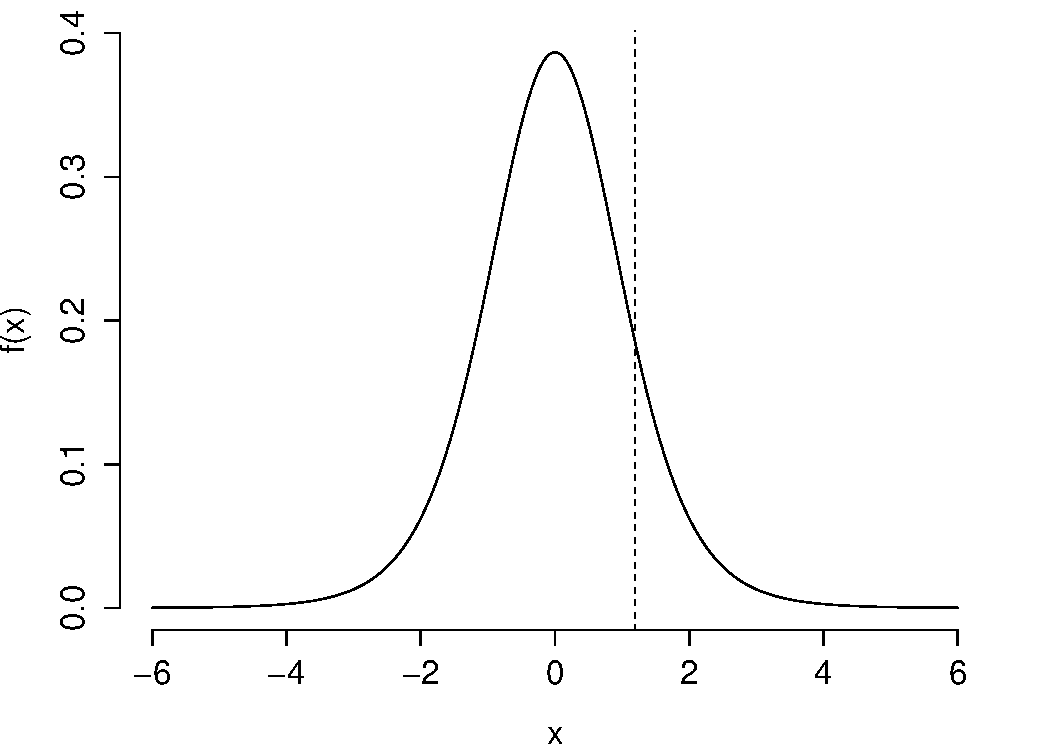
\includegraphics[scale= 0.4]{./images/p_both2}

\end{figure}

\end{frame}

%%%%%%%%%%%%%%%%%%%%%%%%%%%%%%%%%%%%%%%%
\begin{frame}
\frametitle{What is the p-value? (Two-sided Test)}
\footnotesize
Recall: p-value is \emph{smallest significance level} at which our observed test statistic would cause us to reject $H_0$. \alert{Test statistic is $1.14$. What is the two-sided p-value? }
\begin{figure}
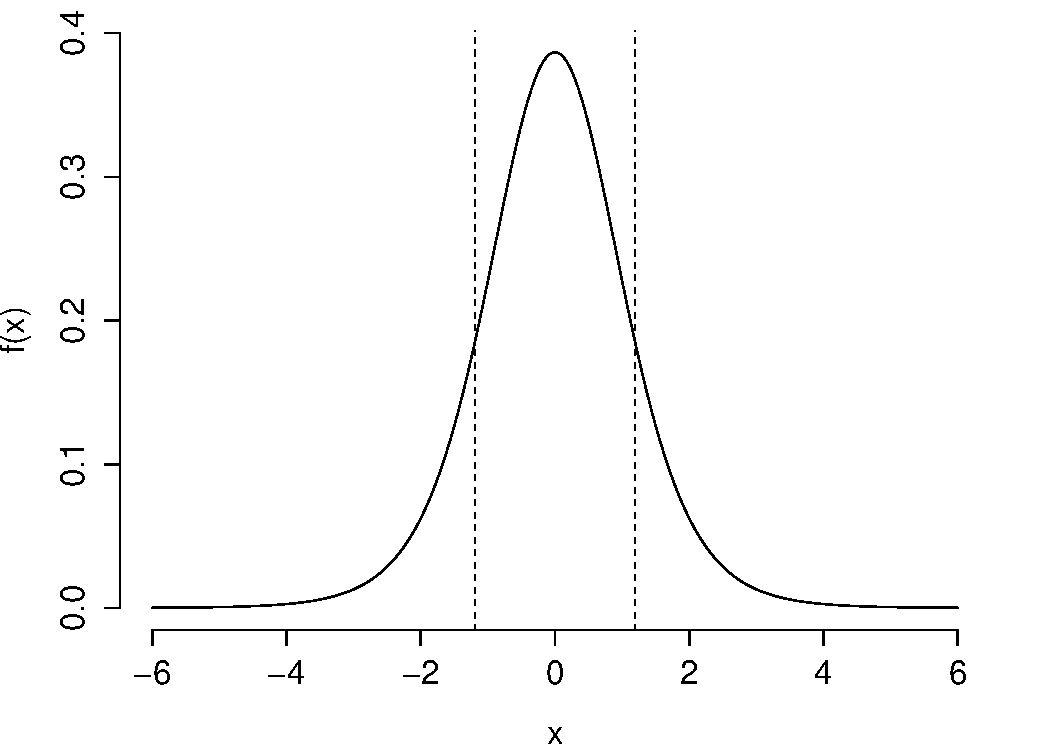
\includegraphics[scale= 0.4]{./images/p_both3}

\end{figure}

\end{frame}

%%%%%%%%%%%%%%%%%%%%%%%%%%%%%%%%%%%%%%%%
\begin{frame}
\frametitle{What is the p-value? (Two-sided Test)}
\footnotesize
Recall: p-value is \emph{smallest significance level} at which our observed test statistic would cause us to reject $H_0$. \alert{Test statistic is $1.14$. What is the two-sided p-value? }
\begin{figure}
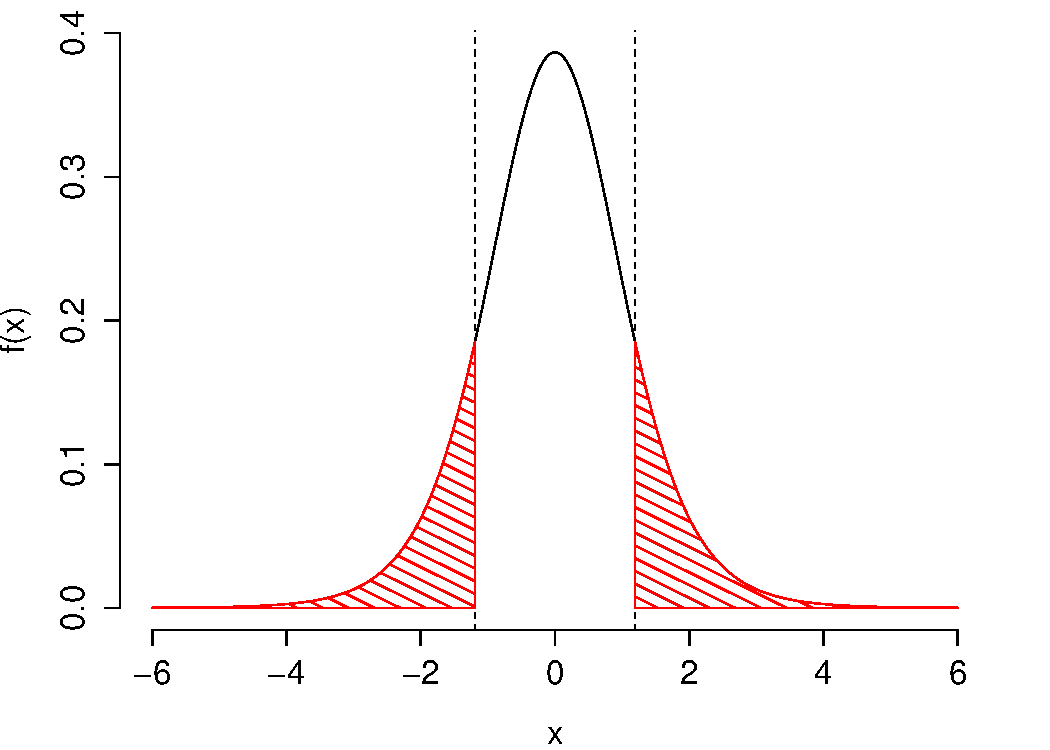
\includegraphics[scale= 0.4]{./images/p_both4}

\end{figure}

\end{frame}

%%%%%%%%%%%%%%%%%%%%%%%%%%%%%%%%%%%%%%%%
\begin{frame}
\frametitle{What is the p-value? (Two-sided Test)}
\footnotesize
Recall: p-value is \emph{smallest significance level} at which our observed test statistic would cause us to reject $H_0$. \alert{Test statistic is $1.14$. What is the two-sided p-value? }
\begin{figure}
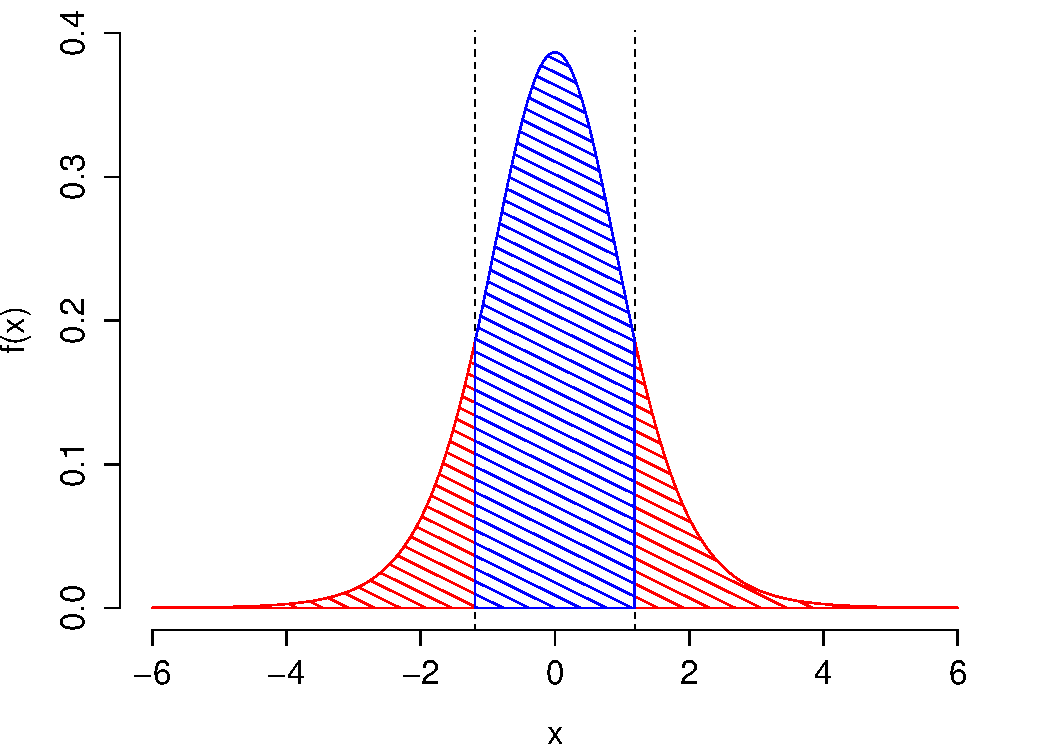
\includegraphics[scale= 0.4]{./images/p_both5}

\end{figure}

\end{frame}

%%%%%%%%%%%%%%%%%%%%%%%%%%%%%%%%%%%%%%%%
\begin{frame}
\frametitle{What is the p-value? (Two-sided Test)}
\footnotesize
Recall: p-value is \emph{smallest significance level} at which our observed test statistic would cause us to reject $H_0$. \alert{Test statistic is $1.14$. What is the two-sided p-value? }
\begin{figure}
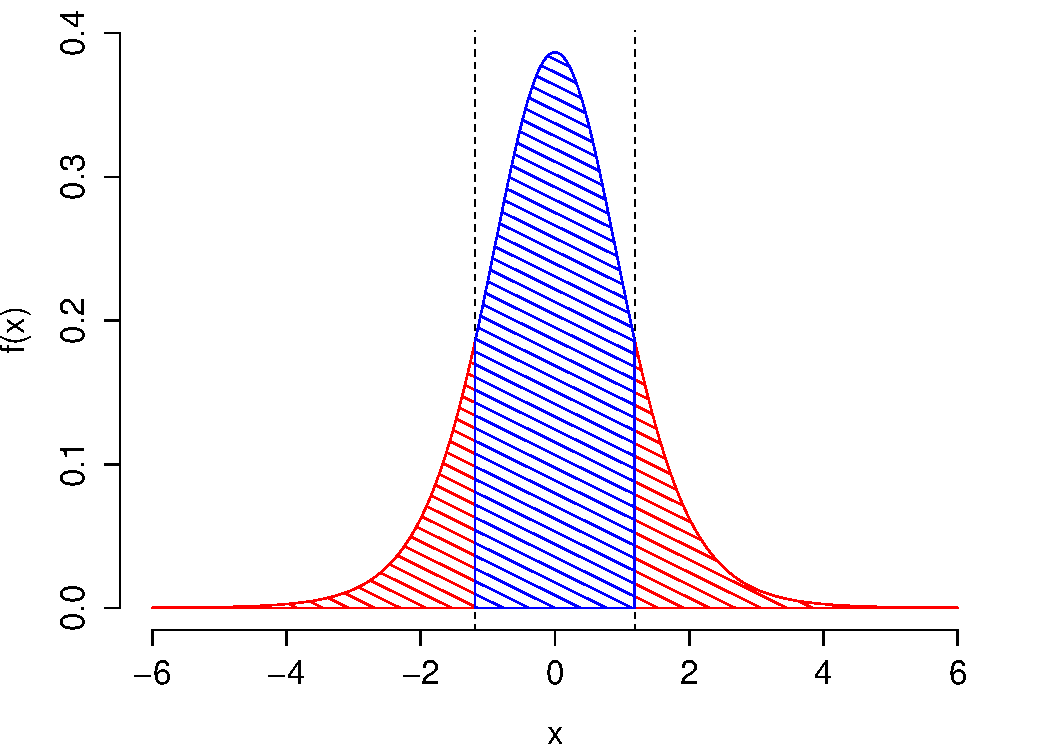
\includegraphics[scale= 0.4]{./images/p_both5}
\end{figure}

\texttt{2 * pt(-1.14, df = 8)}$\approx 0.28$ \pause \hfill \alert{This is twice the one-sided p-value!}
\end{frame}

%%%%%%%%%%%%%%%%%%%%%%%%%%%%%%%%%%%%%%%%

\begin{frame}
\frametitle{Two-sided Test is More Stringent}
\begin{block}{P-value measures strength of evidence against $H_0$}
Lower p-value means stronger evidence. 
\end{block}

\begin{block}{Two Equivalent Definitions of P-value}
	\begin{enumerate}
		\item Smallest significance level at which our observed test statistic would cause us to reject $H_0$.
		\item The probability of observing a test statistic at least as extreme as the one actually observed if $H_0$ were true.
	\end{enumerate}
\end{block}


\begin{block}{(Two-sided p-value) $= 2 \; \times$  (one-sided p-value)}
Reject $H_0$ based on two-sided test $\implies$ Reject $H_0$ based on appropriate one-sided test. The converse is \emph{false}.
\end{block}


\end{frame}
%%%%%%%%%%%%%%%%%%%%%%%%%%%%%%%%%%%%%%%%

\begin{frame}
\begin{center}
\huge P-Value Depends on Which Alternative We Have Specified!
\end{center}
\end{frame}

%%%%%%%%%%%%%%%%%%%%%%%%%%%%%%%%%%%%%%%%
\begin{frame}
\frametitle{Steps in Hypothesis Testing}

\begin{enumerate}
\item Specify Null and Alternative Hypotheses
\item Identify a Test Statistic: a function of the data and the unknown parameter that has a known sampling distribution under the null.
\item Specify a Decision Rule and a Critical Value so the Type I Error Rate equals $\alpha$.
\end{enumerate}

\begin{alertblock}{Alternative to Step 3}
	Calculate P-Value: the minimum significance level  ($\alpha$) at which we would reject $H_0$ given the observed data.
\end{alertblock}

\end{frame}


%%%%%%%%%%%%%%%%%%%%%%%%%%%%%%%%%%%%%%%%
\begin{frame}
\frametitle{How to Handle Other Examples?}

\alert{You already know lots of sampling distributions! Testing is very similar to constructing confidence intervals in that the steps are always the same, and the only thing that differs is \emph{which} sampling distribution we work with.}

\end{frame}

%%%%%%%%%%%%%%%%%%%%%%%%%%%%%%%%%%%%%%%%

%%%%%%%%%%%%%%%%%%%%%%%%%%%%%%%%%%%%%%%%


\begin{frame}
\frametitle{The Anchoring Experiment}
On the first day of class, you were each shown a random number. You were then asked what proportion of UN member states are located in Africa. 

	\begin{block}{``Hi'' Group -- Shown 65 ($n=46$)}
		Sample Mean: $30.7$, Sample Variance: $253$
\end{block}


	\begin{block}{``Lo'' Group -- Shown 10 ($m=43$)}
	Sample Mean: $17.1$, Sample Variance: $86$
\end{block}

\begin{alertblock}{What are we going to test?}
	$H_0\colon \mu_{Lo} = \mu_{Hi}$
\end{alertblock}
\end{frame}
%%%%%%%%%%%%%%%%%%%%%%%%%%%%%%%%%%%%%%%%

\begin{frame}
\frametitle{The Anchoring Experiment}
\begin{figure}
\centering
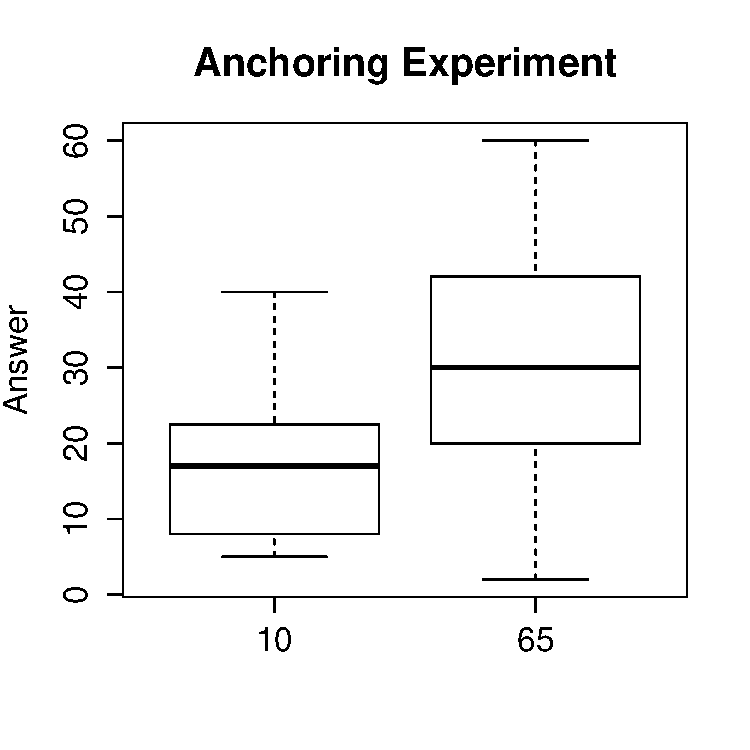
\includegraphics[scale = 0.55]{./images/anchoring_boxplot}
\end{figure}
\end{frame}
%%%%%%%%%%%%%%%%%%%%%%%%%%%%%%%%%%%%%%%%
\begin{frame}
\frametitle{What is our Test Statistic?}
\begin{block}{Sampling Distribution}
		$$\frac{\left(\bar{X}_{Hi} - \bar{X}_{Lo}\right) - \left(\mu_{Hi} - \mu_{Lo}\right)}{\sqrt{\frac{S_{Hi}^2}{n_{Hi}} + \frac{S_{Lo}^2}{n_{Lo}}}} \approx N(0,1)$$
\end{block}

\begin{block}{Test Statistic: Impose the Null}
Under $H_0\colon \mu_{Lo} = \mu_{Hi}$
	$$T_n =\frac{\bar{X}_{Hi} - \bar{X}_{Lo}}{\sqrt{\frac{S_{Hi}^2}{n_{Hi}} + \frac{S_{Lo}^2}{n_{Lo}}}} \approx N(0,1)$$
\end{block}
\end{frame}


%%%%%%%%%%%%%%%%%%%%%%%%%%%%%%%%%%%%%%%%
\begin{frame}
\frametitle{What is our Test Statistic?}
\footnotesize
$\bar{X}_{Hi} = 30.7$, $s^2_{Hi} = 253$, $n_{Hi} = 46$\\
$\bar{X}_{Lo} = 17.1$, $s^2_{Lo} = 86$, $n_{Lo} = 43$\\
\normalsize
\vspace{2em}

\begin{block}{Under $H_0\colon \mu_{Lo} = \mu_{Hi}$}
	$$T_n = \frac{\bar{X}_{Hi} - \bar{X}_{Lo}}{\sqrt{\frac{S_{Hi}^2}{n_{Hi}} + \frac{S_{Lo}^2}{n_{Lo}}}} \approx N(0,1)$$
\end{block}

\begin{block}{Plugging in Our Data}
$$T_n = \frac{\bar{X}_{Hi} - \bar{X}_{Lo}}{\sqrt{\frac{S_{Hi}^2}{n_{Hi}} + \frac{S_{Lo}^2}{n_{Lo}}}} \approx 5$$
\end{block}
\end{frame}


%%%%%%%%%%%%%%%%%%%%%%%%%%%%%%%%%%%%%%%%
\begin{frame}
\frametitle{\hfill 
\includegraphics[scale = 0.05]{./images/clicker}}
Approximately what critical value should we use to test $H_0\colon \mu_{Lo} = \mu_{Hi}$ against the two-sided alternative for this problem?


\vspace{1em}
\begin{center}
\begin{tabular}{l|lll}
$\alpha$ &   0.10& 0.05 &0.01\\
\hline
\texttt{qnorm($1-\alpha$)} & 1.28 &1.64 &2.33\\
\texttt{qnorm($1-\alpha/2$)} &1.64 &1.96& 2.58
\end{tabular}
\end{center}
\vspace{8em}
\end{frame}
%%%%%%%%%%%%%%%%%%%%%%%%%%%%%%%%%%%%%%%%
\begin{frame}
\frametitle{\hfill 
\includegraphics[scale = 0.05]{./images/clicker}}
Which of these commands would give us the p-value of our test of $H_0\colon \mu_{Lo} = \mu$ against $H_1\colon \mu_{Lo}<\mu_{Hi}$ at significance level $\alpha$?
\vspace{1em}
	\begin{enumerate}[(a)]
		\item \texttt{qnorm($1-\alpha$)}
		\item \texttt{qnorm($1-\alpha/2$)}
		\item \texttt{1 - pnorm(5)}
		\item \texttt{2 * (1 - pnorm(5))}
	\end{enumerate}
	

\end{frame}
%%%%%%%%%%%%%%%%%%%%%%%%%%%%%%%%%%%%%%%%

\begin{frame}
\frametitle{P-values for $H_0\colon \mu_{Lo} = \mu_{Hi}$}
We plug in the value of the test statistic that we observed: 5
\begin{block}{Against $H_1\colon \mu_{Lo}< \mu_{Hi}$}
\texttt{1 - pnorm(5)} $< 0.0000$
\end{block}

\begin{block}{Against $H_1\colon \mu_{Lo}\neq \mu_{Hi}$}
\texttt{2 * (1 - pnorm(5))} $< 0.0000$
\end{block}

\vspace{1em}

\alert{If the null is true (the two population means are equal) it would be extremely unlikely to observe a test statistic as large as this!}

\end{frame}

\end{document}